\frontmatter
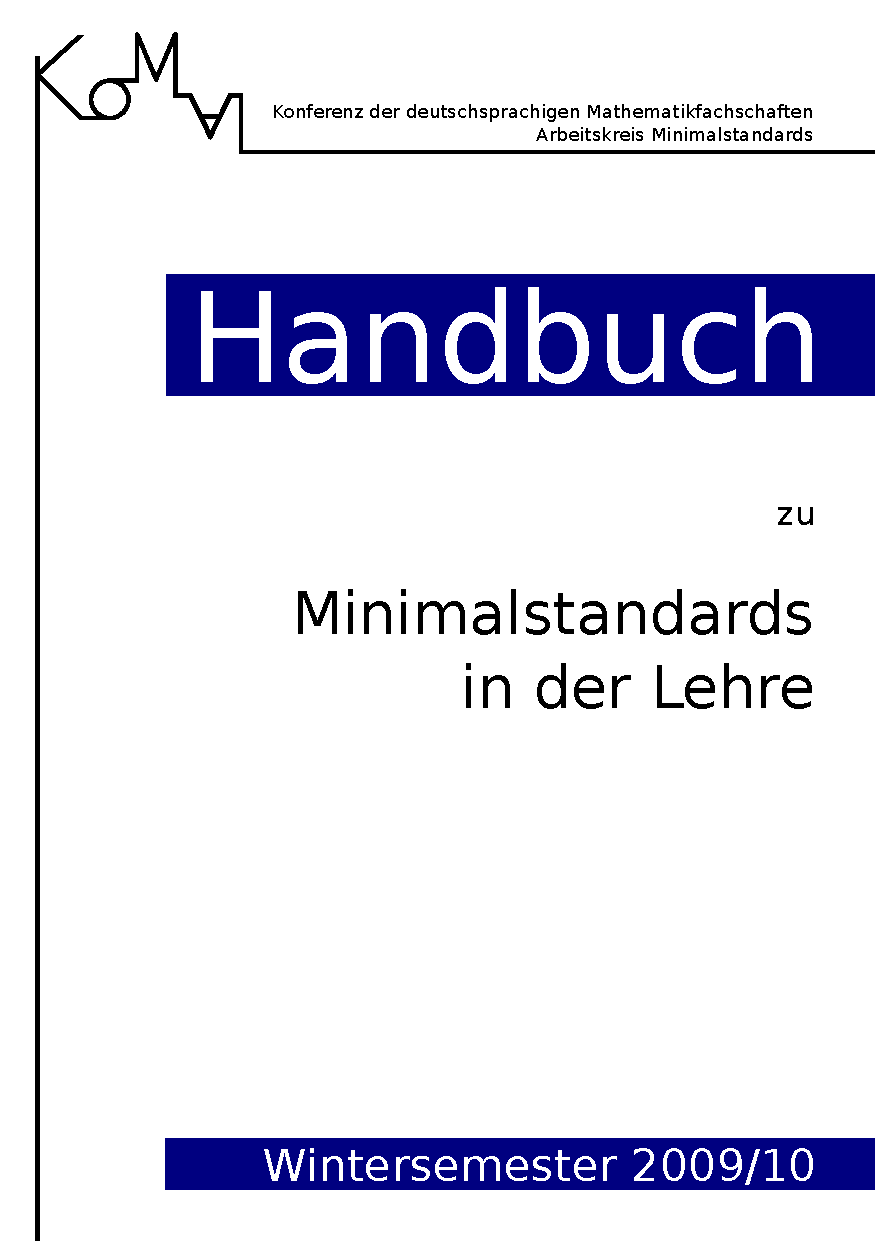
\includegraphics[width=0.8\paperwidth, height=0.8\paperheight]{titelseite}
\newpage
\thispagestyle{empty}
\newpage

\begin{titlepage}
  \begin{flushright}\sffamily
    \vspace*{1cm}
    \Huge{Leitfaden} \\
    \vspace{2.0cm}
    \large{zu}\bigskip\par
    \huge{Minimalstandards in der Lehre} \\
    \vspace*{2ex}
    \vfill
    \large{Arbeitskreis Minimalstandards} \\ 
    \large{der Konferenz der deutschsprachigen Mathematikfachschaften} \\
    \vspace*{1cm}
    \large{erarbeitet auf den Konferenzen} \\	
    {\small
      Bielefeld (WS 06/07), Karlsruhe (SS 07),  \\
      Regensburg (WS 07/08), Chemnitz (SS 08), \\
      Paderborn (WS 08/09), Augsburg (SS 09), \\
      Graz (WS 09/10), Dresden (SS 10)
    } \\
    \vspace*{1cm}
    \large{überarbeitet auf den Konferenzen} \\
    {\small
      Magdeburg (WS 24/25), Passau (SS 25), \\
      Chemnitz (WS 25/26), Münster (WAchKoMa WS 25/26)
    } \\
    \vspace*{2cm}
    {\Large Wintersemester 2025/26}
  \end{flushright}
\end{titlepage}
